\documentclass[12pt]{article}

\usepackage{amsthm}
\usepackage{amsmath}
\usepackage{amssymb}
\usepackage{mathtools}
\usepackage{xcolor}
\usepackage{graphicx}
\usepackage{pgfplots}
\usepackage{hyperref}
\usepackage{url}
\usepackage{minitoc}

\usepackage[left = 1cm, top = 2cm, bottom = 3cm, right = 1cm]{geometry}

\newcommand{\XB}{\color{black}}
\newcommand{\XBB}{\color{blue}}
\newcommand{\XV}{\color{violet}}
\newcommand{\XR}{\color{red}}
\newcommand{\ds}{\displaystyle}

\setcounter{secnumdepth}{0}

\begin{document}

\title{\textbf{CSC517}: Social Computing - \\ Non-mainstream social tool for a specific community: \\ All Trails}
\date{\today}
\author{\XV\textit{\large{\href{https://github.com/casonk}{Cason Konzer}}}\XB}

\maketitle
\hrulefill
\vfill 

\pagebreak

\tableofcontents
% \listoftables
\listoffigures

\newpage

\section{Narrative Report}
The tool I have chosen for non-mainstream social computing is called All Trails.
I came across this tool while starting off my undergraduate degree at Westminster College in Salt Lake City, UT. 
In the area there was a plethora of stunning trails and hikes, but the challenge was always finding them. 
I found this tool on the Apple App Store in hopes to find new trails relative to my vacation destinations and weekend plans. 
For the UI I will be sharing the web version, the home page is shown in Figure~\ref{fig:AT_Home}. 

All Trails is intended not just for hiking, but also mountain biking, trail running, backpacking, and walking. 
The company is focused on curating outdoor experiences and cleaning up our natural resources.
A comprehensive list of their values is shown in Figure~\ref{fig:AT_Values}, with additional details on community works available at the cited page. 
The main use cases for All Trails are trail selection and trail discovery, while additionally bringing together trail enthusiasts. 
Access to All Trails can be made through either mobile apps or a browser. 
When and where the tool is used is ambiguous, it could that you are looking for a quick excursion in your local area, or otherwise planning for an upcoming trip. 

In order to preview the features of the tool we will take an example trail - \emph{Holly State Recreation Area Wilderness Trail}: Figure~\ref{fig:AT_HSRAWT1}.
From the overview we can see some key information about the trail such as length, elevation gain, and route type. 
A brief description of the trail is given, along with tags and an overhead map view. 
Personally, a key feature was the photos (Figure~\ref{fig:AT_HSRAWT_Photos}) and reviews (Figure~\ref{fig:AT_HSRAWT_Reviews}). 
For community features you can follow local users, make posts, and like and comment on posts (Figure~\ref{fig:AT_Community}). 
Concluding, this tool is for looking at upcoming trails, and sharing experiences from past trails. 

\newpage

\section{Appendix : Figures}

\begin{figure}[ht!]
    \centering
    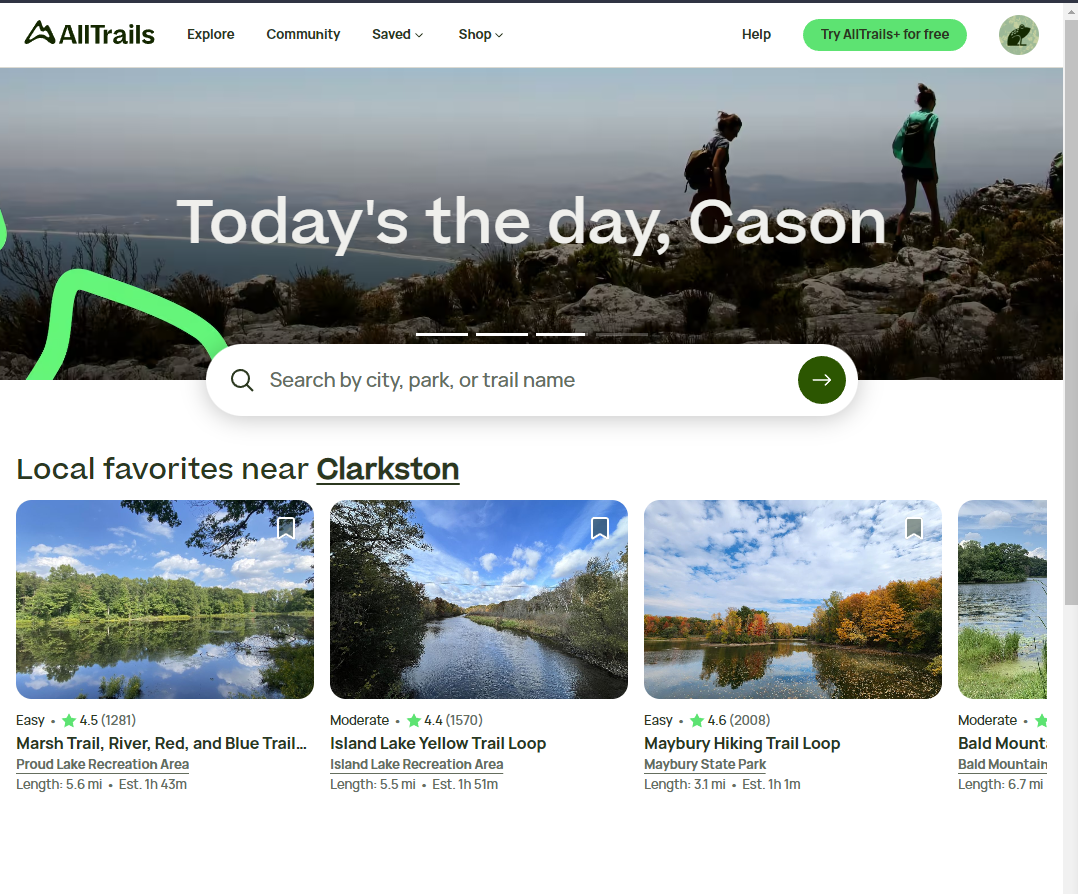
\includegraphics[width=\textwidth]{./AT_Home.PNG}
    \caption{All Trails: Home Page - \url{https://www.alltrails.com/}}
    \label{fig:AT_Home}
\end{figure}

\begin{figure}[ht!]
    \centering
    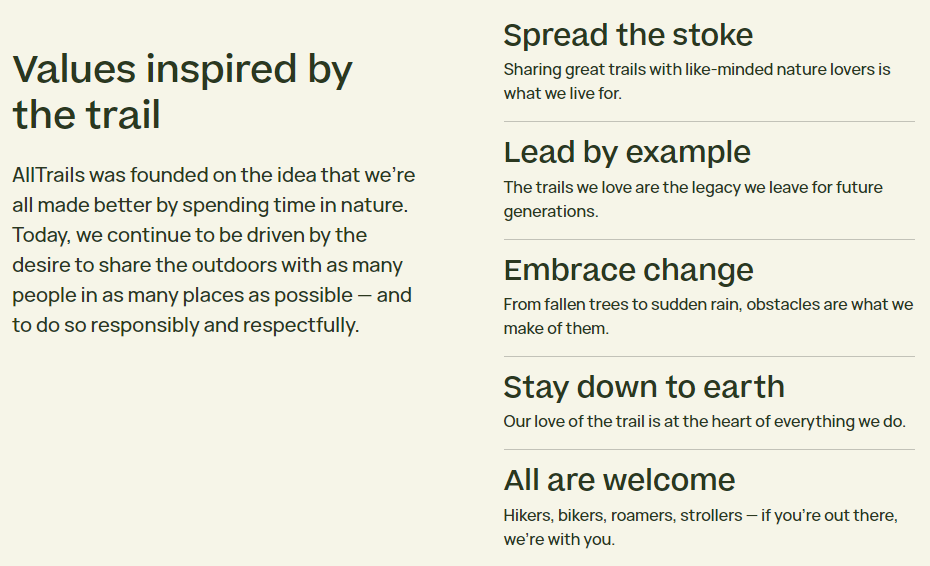
\includegraphics[width=\textwidth]{./AT_Values.PNG}
    \caption{All Trails: About - \url{https://www.alltrails.com/about}}
    \label{fig:AT_Values}
\end{figure}

\begin{figure}[ht!]
    \centering
    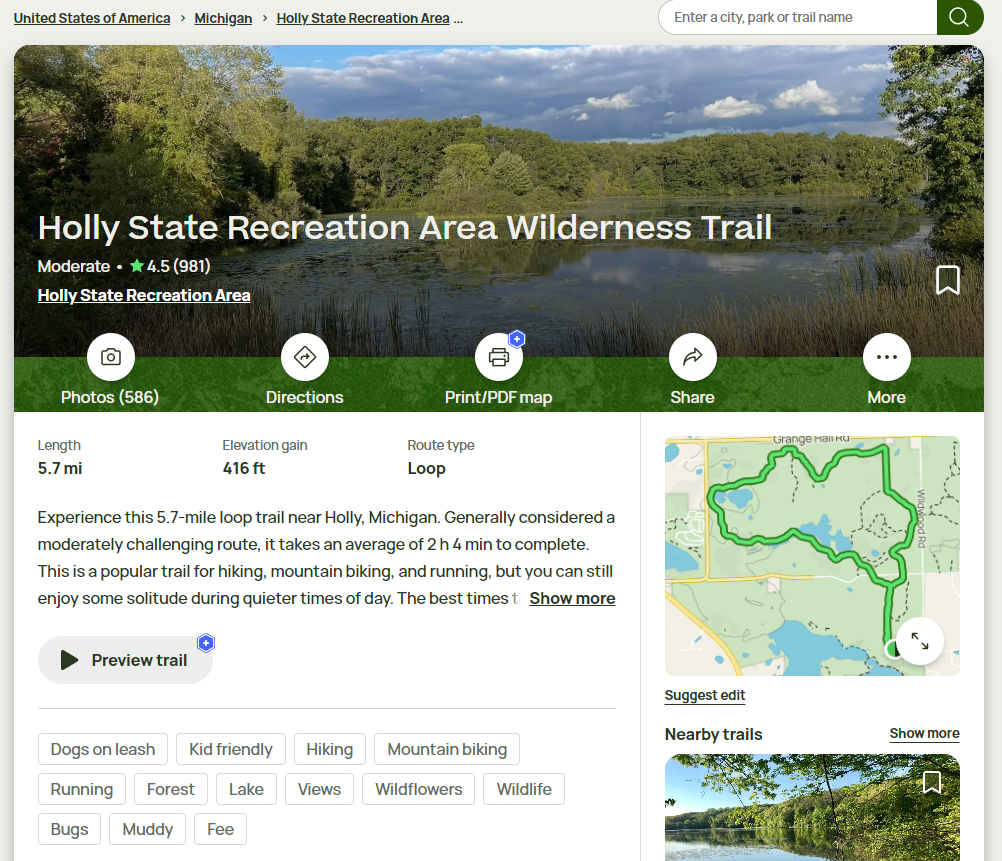
\includegraphics[width=\textwidth]{./AT_HSRAWT1.PNG}
    \caption{All Trails: Holly State Recreation Area Wilderness Trail - \url{https://www.alltrails.com/trail/us/michigan/holly-state-recreation-area-wilderness-trail}}
    \label{fig:AT_HSRAWT1}
\end{figure}

\begin{figure}[ht!]
    \centering
    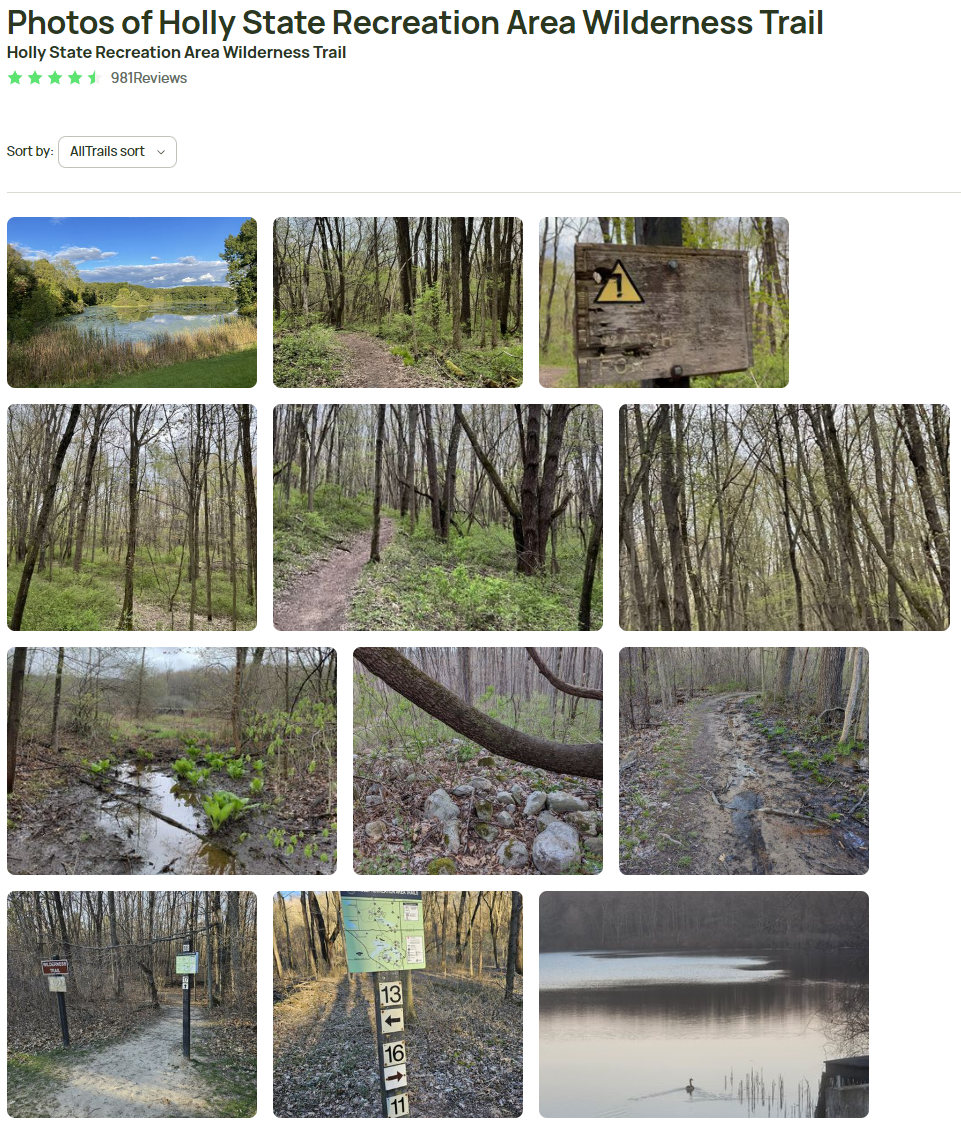
\includegraphics[width=0.9\textwidth]{./AT_HSRAWT_Photos.PNG}
    \caption{All Trails: Photos of Holly State Recreation Area Wilderness Trail - \url{https://www.alltrails.com/trail/us/michigan/holly-state-recreation-area-wilderness-trail/photos}}
    \label{fig:AT_HSRAWT_Photos}
\end{figure}

\begin{figure}[ht!]
    \centering
    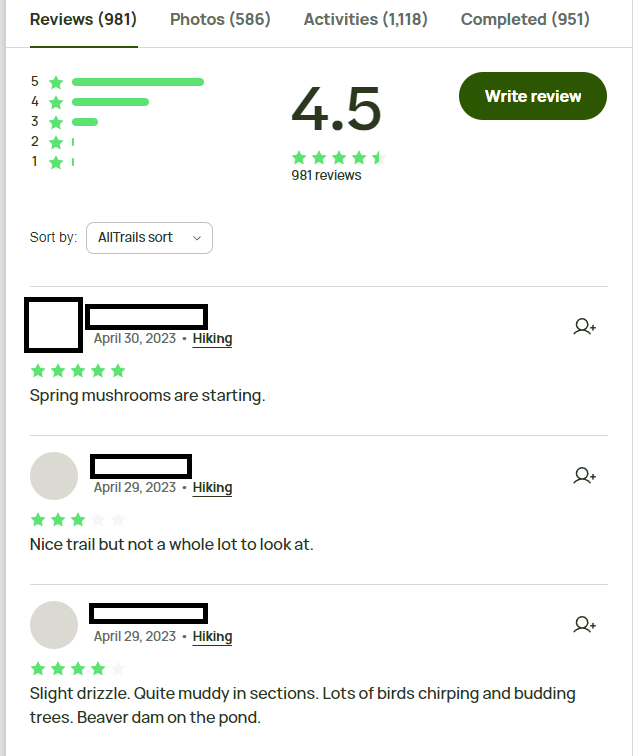
\includegraphics[width=0.9\textwidth]{./AT_HSRAWT_Reviews.PNG}
    \caption{All Trails: Holly State Recreation Area Wilderness Trail - Reviews}
    \label{fig:AT_HSRAWT_Reviews}
\end{figure}

\begin{figure}[ht!]
    \centering
    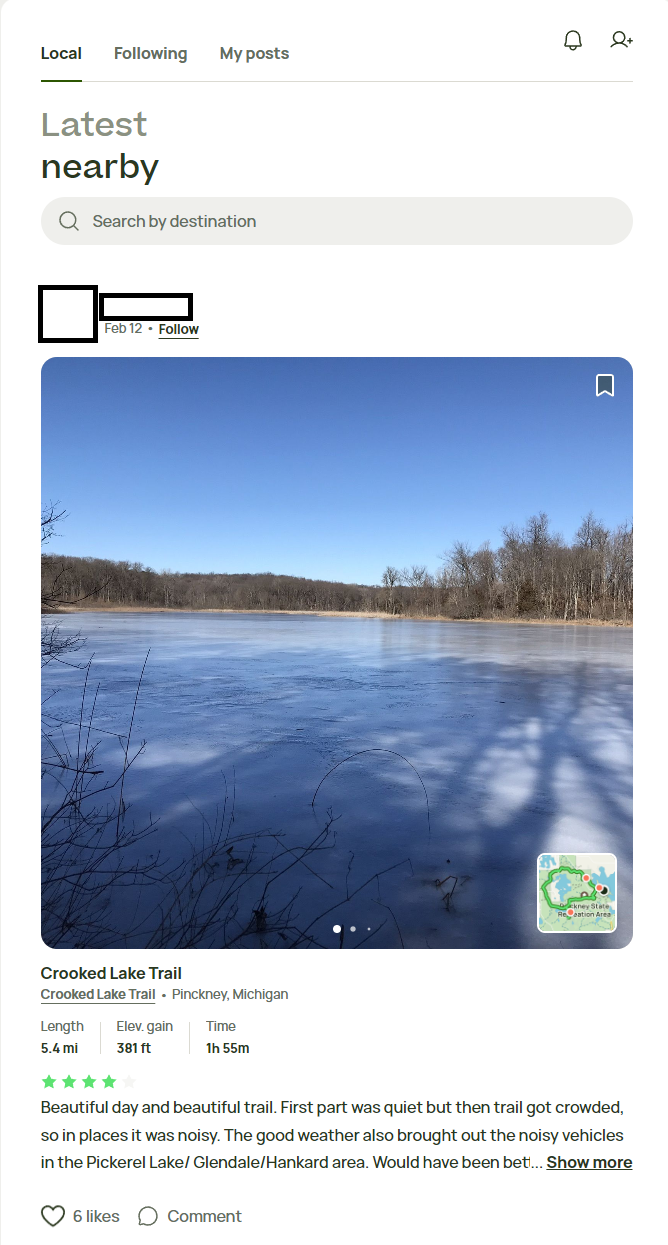
\includegraphics[width=0.5\textwidth]{./AT_Community.PNG}
    \caption{All Trails: Community - \url{https://www.alltrails.com/community}}
    \label{fig:AT_Community}
\end{figure}

\end{document}